%%%%%%%%%%%%%%%%%%%%%%%%%%%%%%%%%%%%%%%%%
% Short Sectioned Assignment LaTeX Template Version 1.0 (5/5/12)
% This template has been downloaded from: http://www.LaTeXTemplates.com
% Original author:  Frits Wenneker (http://www.howtotex.com)
% License: CC BY-NC-SA 3.0 (http://creativecommons.org/licenses/by-nc-sa/3.0/)
%%%%%%%%%%%%%%%%%%%%%%%%%%%%%%%%%%%%%%%%%

%----------------------------------------------------------------------------------------
%	PACKAGES AND OTHER DOCUMENT CONFIGURATIONS
%----------------------------------------------------------------------------------------

\documentclass[paper=a4, fontsize=11pt]{scrartcl} % A4 paper and 11pt font size

% ---- Entrada y salida de texto -----

\usepackage[T1]{fontenc} % Use 8-bit encoding that has 256 glyphs
\usepackage[utf8]{inputenc}
%\usepackage{fourier} % Use the Adobe Utopia font for the document - comment this line to return to the LaTeX default

% ---- Idioma --------

\usepackage[spanish, es-tabla]{babel} % Selecciona el español para palabras introducidas automáticamente, p.ej. "septiembre" en la fecha y especifica que se use la palabra Tabla en vez de Cuadro

% ---- Otros paquetes ----

\usepackage{url} % ,href} %para incluir URLs e hipervínculos dentro del texto (aunque hay que instalar href)
\usepackage{amsmath,amsfonts,amsthm} % Math packages
%\usepackage{graphics,graphicx, floatrow} %para incluir imágenes y notas en las imágenes
\usepackage{graphics,graphicx, float} %para incluir imágenes y colocarlas

% Para hacer tablas comlejas
%\usepackage{multirow}
%\usepackage{threeparttable}

%\usepackage{sectsty} % Allows customizing section commands
%\allsectionsfont{\centering \normalfont\scshape} % Make all sections centered, the default font and small caps

\usepackage{fancyhdr} % Custom headers and footers
\pagestyle{fancyplain} % Makes all pages in the document conform to the custom headers and footers
\fancyhead{} % No page header - if you want one, create it in the same way as the footers below
\fancyfoot[L]{} % Empty left footer
\fancyfoot[C]{} % Empty center footer
\fancyfoot[R]{\thepage} % Page numbering for right footer
\renewcommand{\headrulewidth}{0pt} % Remove header underlines
\renewcommand{\footrulewidth}{0pt} % Remove footer underlines
\setlength{\headheight}{13.6pt} % Customize the height of the header

\numberwithin{equation}{section} % Number equations within sections (i.e. 1.1, 1.2, 2.1, 2.2 instead of 1, 2, 3, 4)
\numberwithin{figure}{section} % Number figures within sections (i.e. 1.1, 1.2, 2.1, 2.2 instead of 1, 2, 3, 4)
\numberwithin{table}{section} % Number tables within sections (i.e. 1.1, 1.2, 2.1, 2.2 instead of 1, 2, 3, 4)

\setlength\parindent{0pt} % Removes all indentation from paragraphs - comment this line for an assignment with lots of text

\newcommand{\horrule}[1]{\rule{\linewidth}{#1}} % Create horizontal rule command with 1 argument of height

\usepackage{graphicx}
\graphicspath{ {./imgs/} }

%----------------------------------------------------------------------------------------
%	TÍTULO Y DATOS DEL ALUMNO
%----------------------------------------------------------------------------------------

\title{	
	\normalfont \normalsize 
	\textsc{\textbf{Inteligencia de Negocio (2018-2019)} \\ Doble Grado en Ingeniería Informática y Matemáticas \\ Universidad de Granada} \\ [25pt] % Your university, school and/or department name(s)
	\horrule{0.5pt} \\[0.4cm] % Thin top horizontal rule
	\huge Memoria Práctica 3: \\ Competición en DrivenData. Grupo de Prácticas 1 \\ % The assignment title
	\horrule{2pt} \\[0.5cm] % Thick bottom horizontal rule
}

\author{Luis Balderas Ruiz \\ \texttt{luisbalderas@correo.ugr.es}} 
% Nombre y apellidos 

\date{\normalsize\today} % Incluye la fecha actual

%----------------------------------------------------------------------------------------
% DOCUMENTO
%----------------------------------------------------------------------------------------

\begin{document}
	
\maketitle % Muestra el Título
	
\newpage %inserta un salto de página

\section{Posición en la competición y entregas}	

\begin{figure}[H] %con el [H] le obligamos a situar aquí la figura
	\centering
	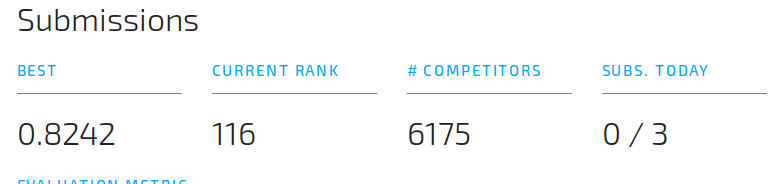
\includegraphics[scale=0.5]{rank.png}  %el parámetro scale permite agrandar o achicar la imagen. En el nombre de archivo puede especificar directorios
	\caption{Posición final el día 6 de enero a las 00:00} 
	\label{fig:rank}
\end{figure}
	
	
\begin{figure}[H] %con el [H] le obligamos a situar aquí la figura
	\centering
	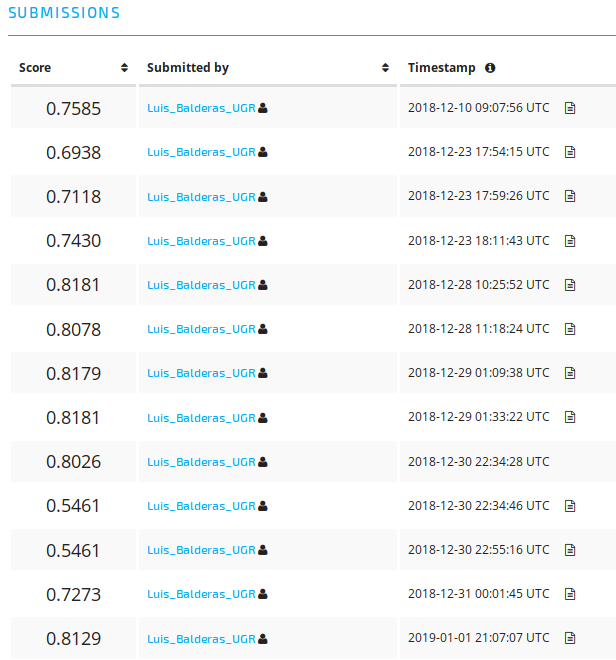
\includegraphics[scale=0.5]{sub1.png}  %el parámetro scale permite agrandar o achicar la imagen. En el nombre de archivo puede especificar directorios
	\caption{Entregas (1)} 
	\label{fig:sub1}
\end{figure}
	
	
\begin{figure}[H] %con el [H] le obligamos a situar aquí la figura
	\centering
	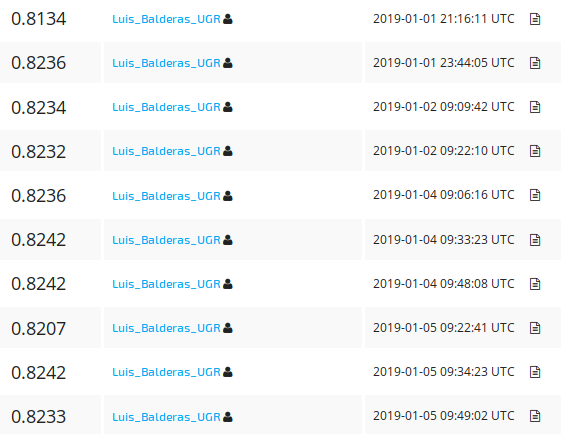
\includegraphics[scale=0.5]{sub2.png}  %el parámetro scale permite agrandar o achicar la imagen. En el nombre de archivo puede especificar directorios
	\caption{Entregas (2)} 
	\label{fig:sub2}
\end{figure}

\newpage
	
\tableofcontents % para generar el índice de contenidos
	
\listoffigures

	
\newpage



%----------------------------------------------------------------------------------------
%	Introducción
%----------------------------------------------------------------------------------------

\section{Introducción}

En la presente práctica nos hemos enfrentado a la competición de Driven Data \textit{Pump it Up: Data Mining the Water Table} basada en predecir qué bombas de extracción de aguas funcionan, cuáles necesitan algunas reparaciones y cuáles no funcionan. Para predecir una de estas tres clases se dispone de 39 variables sobre qué tipo de bomba se está usando, cuándo se instaló, cómo se administra, su ubicación, datos sobre la cuenca geográfica, tipo de extracción, coste del agua,etcc. Una comprensión inteligente de qué puntos de agua fallarán puede mejorar las operaciones de mantenimiento y garantizar que el agua potable y limpia esté disponible para las comunidades de Tanzania. El conjunto de entrenamiento consta de 59.400 instancias. \\

En mi caso, para cumplir las restricciones impuestas en el guión, incluyo en la documentación cuatro directorios que las soluciones que he desarrollado. El primero, llamado \textit{Pruebas}, contiene dos ficheros en los que, utilizando el código de ejemplo del profesor D. Jorge Casillas, pongo en práctica otros algoritmos como son Random Forest y XGB. Tras familiarizarme con el problema, pasé a desarrollar una de mis soluciones. Dicha solución se encuentra en \textit{Solucion 1} y hago un preprocesamiento más exhaustivo para finalmente utilizar Random Forest. Sobre esta hago ciertas modificaciones en parámetros y preprocesamiento (introduzco PCA, elimino unas variables a veces y otras no) para ver cómo se comporta el score. Para esta solución, mi score más alto es 0.8181 (puesto 476). \\

Sin embargo, al tratarse de un problema multiclase, sospecho que Random Forest puede flojear, así que intento acercarme a algoritmos de boosting tipo XGB o uno nuevo que descubro en la literatura llamado CatBoost. El intento fue fallido (\textit{Solución 2}). Por tanto, vuelvo a mi anterior RF para intentar mejorar la puntuación cambiando de nuevo parámetros e intentando nuevos preprocesamientos. \\

Ante la falta de mejora, comienzo totalmente de nuevo el problema (Solución 3). Cambio de Python a R ya que echaba en falta la facilidad que da R para visualizar tablas y conjuntos de datos además de la inmediatez de la selección de características. Tras un preprocesamiento basado en eliminar aquellas columnas que parecen no mejorar la clasificación, tratamiento de valores perdidos de algunas variables y modificación del formato de otras. Una vez procesados, utilizo un XGB con validación cruzada para determinar cuántas veces ejecuto el modelo. Tras varios ajustes sobre el algoritmo consigo mi mayor puntuación (0.8242, puesto 114). \\

Para acabar quiero reseñar que fundamentalmente he basado mi solución en las técnicas aprendidas en clase, en \cite{data_mining_book}, \cite{sklearn} y \cite{foro}


\section{Tabla resumen}

Presento la tabla resumen de todas las subidas. Muchas de ellas parten de un preprocesamiento general para luego ir haciendo pequeñas modificaciones en parámetros. Por tanto, no repetiré la descripción en cada entrada, sino cuando sea realmente novedoso para así facilitar la escritura e interpretación de la tabla. 


\begin{table}[H]
	\resizebox{16cm}{13cm}{
	\begin{tabular}{|c|c|c|c|c|c|c|c|c|}
		\hline
		\textbf{Solución} & \textbf{Fecha y Hora} & \textbf{Posición} & \textbf{Score Training} & \textbf{Score Driven Data} & \textbf{Descripción Preprocesado}                                                                                                                                                                                                                                                                                                                                                                                                                                                                                                                                                                                                                                       & \textbf{Descripción Clasificador}                       & \textbf{\begin{tabular}[c]{@{}c@{}}Configuración\\ Parámetros\end{tabular}}                                                                                                                                                                                                         & \textbf{Título}                                                                                                    \\ \hline
		Pruebas           & 2018-12-10 10:07:56   & 1377              & 0.825                   & 0.7585                     & Ninguno                                                                                                                                                                                                                                                                                                                                                                                                                                                                                                                                                                                                                                                                 & LightGBM                                                & \begin{tabular}[c]{@{}c@{}}200 estimadores\\ 2 hebras\end{tabular}                                                                                                                                                                                                                  & \begin{tabular}[c]{@{}c@{}}Código de prueba\\ de Jorge Casillas\end{tabular}                                       \\ \hline
		Pruebas           & 23/12/2018 – 18:55    & 1397              & 0.6932                  & 0.6938                     & Ninguno                                                                                                                                                                                                                                                                                                                                                                                                                                                                                                                                                                                                                                                                 & Random Forest                                           & \begin{tabular}[c]{@{}c@{}}200 estimadores\\ max\_depth=5\end{tabular}                                                                                                                                                                                                              & \begin{tabular}[c]{@{}c@{}}Probando con\\ Random Forest\end{tabular}                                               \\ \hline
		Pruebas           & 23/12/2018-18:59      & 1397              & 0.7131                  & 0.7118                     & \begin{tabular}[c]{@{}c@{}}Imputación de valores\\ perdidos a través del más\\ frecuente\end{tabular}                                                                                                                                                                                                                                                                                                                                                                                                                                                                                                                                                                   & Random Forest                                           & \begin{tabular}[c]{@{}c@{}}200 estimadores\\ max\_depth=5\end{tabular}                                                                                                                                                                                                              & \begin{tabular}[c]{@{}c@{}}Imputando valores\\ perdidos en RF\end{tabular}                                         \\ \hline
		Pruebas           & 23/12/2018 – 19:11    & 1397              & 0.7647                  & 0.743                      & Ninguno                                                                                                                                                                                                                                                                                                                                                                                                                                                                                                                                                                                                                                                                 & XGBoost sin CV                                          & 200 estimadores                                                                                                                                                                                                                                                                     & \begin{tabular}[c]{@{}c@{}}Probando el código\\ comentado del \\ \\ ejemplo\end{tabular}                           \\ \hline
		Solución 1        & 2018-12-28 11:25:52   & 476               & 0.82                    & 0.8181                     & \begin{tabular}[c]{@{}c@{}}- Modificación del formato date\\ - Tratamiento de valores perdidos en \\ \\ 'construction\_year' (35\% son v.p. -\textgreater imputo\\ la media)\\ - Cambio Null por False en 'public\_meeting' y\\ 'permit'\\ - Null de 'longitude', 'latitude', 'gps\_height',\\ 'population' se cambian por las medias.\\ - 'region\_code', 'district\_code' a string\\ - Eliminación de 'id','amount\_tsh',  'num\_private', 'region',\\ 'quantity', 'quality\_group', 'source\_type', 'payment',\\ 'waterpoint\_type\_group', 'extraction\_type\_group'\\ - LDA sobre 'population', 'gps\_height', 'latitude', 'longitude'\\ \\ - Dummies\end{tabular} & Random Forest                                           & \begin{tabular}[c]{@{}c@{}}Estimación de \\ \\ hiperparámetros\\ con GridSearch. \\ \\ Mejores resultados:\\ 1000 estimadores.\\ \\ \\ Criterio:gini\\ min\_samples\_split=6\\ max\_features='auto',\\ oob\_score=True,\\ n\_jobs=-1\end{tabular}                                   & \begin{tabular}[c]{@{}c@{}}Preprocesamiento\\ profundo con RF\\ y ajuste de hiperparámetros\end{tabular}           \\ \hline
		Solución 1        & 2018-12-28 12:18:24   & 476               & 0.81                    & 0.8078                     & Idem                                                                                                                                                                                                                                                                                                                                                                                                                                                                                                                                                                                                                                                                    & LightGBM                                                & \begin{tabular}[c]{@{}c@{}}Objetive:binary\\ num\_estimadores=1000\end{tabular}                                                                                                                                                                                                     & \begin{tabular}[c]{@{}c@{}}Cambiando a un nuevo\\ algoritmo para ver mejoría\end{tabular}                          \\ \hline
		Solución 1        & 2018-12-29 02:09:38   & 476               & 0.8129                  & 0.8179                     & Idem añadiendo codes                                                                                                                                                                                                                                                                                                                                                                                                                                                                                                                                                                                                                                                    & Random Forest                                           & 500 estimadores                                                                                                                                                                                                                                                                     & \begin{tabular}[c]{@{}c@{}}Sobre RF, agregar\\ pequeñas modificaciones\\ en preprocesamiento\end{tabular}          \\ \hline
		Solución 1        & 2018-12-29 02:33:22   & 476               & 0.8136                  & 0.8181                     & \begin{tabular}[c]{@{}c@{}}Idem cambiando LDA por\\ PCA\end{tabular}                                                                                                                                                                                                                                                                                                                                                                                                                                                                                                                                                                                                    & \begin{tabular}[c]{@{}c@{}}Random\\ Forest\end{tabular} & 500 estimadores                                                                                                                                                                                                                                                                     & Probando con PCA                                                                                                   \\ \hline
		Solución 2        & 2018-12-30 23:34:28   & 476               & 0.82                    & 0.8026                     & \begin{tabular}[c]{@{}c@{}}-Eliminar características con\\ muy pocos o muchos valores distintos\\ -Reemplazamiento de NaN\\ - Reemplazamiento de 0\\ - Imputación de MV\\ - Codificación de variables categóricas\\ - Escalar características\end{tabular}                                                                                                                                                                                                                                                                                                                                                                           & CatBoost                                                & \begin{tabular}[c]{@{}c@{}}Learning\_rate=0.1\\ loss\_function = MultiClass\\ eval\_metric = Accuracy\\ od\_pval=0.01\end{tabular}                                                                                                                                                  & \begin{tabular}[c]{@{}c@{}}Investigando con \\ \\ CatBoost\end{tabular}                                            \\ \hline
		Solución 2        & 2018-12-30 23:34:46   & 476               & 0.6                     & 0.5461                     & Idem                                                                                                                                                                                                                                                                                                                                                                                                                                                                                                                                                                                                                                                                    & XGBoost                                                 & \begin{tabular}[c]{@{}c@{}}'booster': 'gbtree',\\         'objective': 'multi:softmax',\\         'eta': 0.025,\\         'max\_depth': 23,\\         'colsample\_bytree': 0.4,\\         'silent': 1,\\         'eval\_metric': 'mlogloss',\\         'num\_class': 3\end{tabular} & \begin{tabular}[c]{@{}c@{}}Intento muy fallido\\ con XGBoost.\\ Probables errores\\ no encontrados\end{tabular}    \\ \hline
		Solución 2        & 2018-12-30 23:55:16   & 476               & 0.65                    & 0.5461                     & Idem                                                                                                                                                                                                                                                                                                                                                                                                                                                                                                                                                                                                                                                                    & XGBoost                                                 & Idem. 'eta':0.1                                                                                                                                                                                                                                                                     & \begin{tabular}[c]{@{}c@{}}Intentando mejorar\\ resultados sin éxito\end{tabular}                                  \\ \hline
		Solución 2        & 2018-12-31 01:01:45   & 476               & 0.79                    & 0.7273                     & Idem                                                                                                                                                                                                                                                                                                                                                                                                                                                                                                                                                                                                                                                                    & XGBoost                                                 & Idem                                                                                                                                                                                                                                                                                & \begin{tabular}[c]{@{}c@{}}Corrigiendo errata\\ que hace mejorar \\ \\ pero no suficiente\end{tabular}             \\ \hline
		Solución 1        & 01/01/2019 21:07:00   & 476               & 0.8083                  & 0.8129                     & \begin{tabular}[c]{@{}c@{}}Mismo preprocesamiento\\ que en 8 pero sin eliminar\\ 'population' ni 'installer'\end{tabular}                                                                                                                                                                                                                                                                                                                                                                                                                                                                                                                                               & \begin{tabular}[c]{@{}c@{}}Random\\ Forest\end{tabular} & 1000 estimadores                                                                                                                                                                                                                                                                    & \begin{tabular}[c]{@{}c@{}}Volviendo a mi\\ mejor solución buscando\\ progresar\end{tabular}                       \\ \hline
		Solución 1        & 01/01/2019 21:16:00   & 476               & 0.8086                  & 0.8134                     & Idem                                                                                                                                                                                                                                                                                                                                                                                                                                                                                                                                                                                                                                                                    & \begin{tabular}[c]{@{}c@{}}Random\\ Forest\end{tabular} & 500 estimadores                                                                                                                                                                                                                                                                     & \begin{tabular}[c]{@{}c@{}}Disminuyendo\\ el número de\\  estimadores\end{tabular}                                 \\ \hline
		Solución 3        & 2019-01-02 00:44:05   & 146               & 0.83                    & 0.8236                     & \begin{tabular}[c]{@{}c@{}}- Reducción de 40 a 26 \\ \\ variables por similitud.\\ - Imputación de MV y 0 \\ \\ en 'construction\_year' y \\ \\ 'gps\_height'.\end{tabular}                                                                                                                                                                                                                                                                                                                                                                                                                                                                                             & XGBoost                                                 & \begin{tabular}[c]{@{}c@{}}objective = "multi:softmax", \\ \\ booster = "gboost"\\ eval\_metric = "merror", \\ nrounds = min.error.idx, \\ \\  num\_class = 4,\\ eta = .2, \\ \\ max\_depth = 12, \\ \\ colsample\_bytree = .4\end{tabular}                                         & \begin{tabular}[c]{@{}c@{}}Nueva solución con\\ XGBoost ahora sí\\ efectiva\end{tabular}                           \\ \hline
		Solución 3        & 2019-01-02 10:09:42   & 146               & 0.825                   & 0.8234                     & Idem sin eliminar 'installer'                                                                                                                                                                                                                                                                                                                                                                                                                                                                                                                                                                                                                                           & XGBoost                                                 & Idem                                                                                                                                                                                                                                                                                & Nuevo descenso                                                                                                     \\ \hline
		Solución 3        & 2019-01-02 10:22:10   & 146               & 0.82                    & 0.8232                     & \begin{tabular}[c]{@{}c@{}}Vuelta al preprocesado\\ anterior\end{tabular}                                                                                                                                                                                                                                                                                                                                                                                                                                                                                                                                                                                               & XGBoost                                                 & Número de iteraciones a 10                                                                                                                                                                                                                                                          & \begin{tabular}[c]{@{}c@{}}Cambiando el número \\ \\ de iteraciones que \\ \\ se ejecuta el algoritmo\end{tabular} \\ \hline
		Solución 3        & 2019-01-04 10:06:16   & 147               & 0.825                   & 0.8236                     & Idem                                                                                                                                                                                                                                                                                                                                                                                                                                                                                                                                                                                                                                                                    & XGBoost                                                 & \begin{tabular}[c]{@{}c@{}}12 iteraciones\\ 'eta':0.2\end{tabular}                                                                                                                                                                                                                  & \begin{tabular}[c]{@{}c@{}}Probando distintas \\ \\ configuraciones\end{tabular}                                   \\ \hline
		Solución 3        & 2019-01-04 10:33:23   & 114               & 0.827                   & 0.8242                     & Idem                                                                                                                                                                                                                                                                                                                                                                                                                                                                                                                                                                                                                                                                    & XGBoost                                                 & \begin{tabular}[c]{@{}c@{}}20 iteraciones\\ 'eta':0.3\end{tabular}                                                                                                                                                                                                                  & \begin{tabular}[c]{@{}c@{}}Mejor resultado\\ de mi competición\end{tabular}                                        \\ \hline
		Solución 3        & 2019-01-04 10:48:41   & 114               & 0.835                   & 0.8242                     & Idem                                                                                                                                                                                                                                                                                                                                                                                                                                                                                                                                                                                                                                                                    & XGBoost                                                 & \begin{tabular}[c]{@{}c@{}}25 iteraciones\\ 'eta':0.35\\ max\_depth=14\end{tabular}                                                                                                                                                                                                 & \begin{tabular}[c]{@{}c@{}}Intentado\\ subir al top 100\end{tabular}                                               \\ \hline
		Solución 3        & 2019-01-05 10:22:41   & 116               & 0.835                   & 0.8207                     & Idem                                                                                                                                                                                                                                                                                                                                                                                                                                                                                                                                                                                                                                                                    & XGBoost                                                 & \begin{tabular}[c]{@{}c@{}}20 iteraciones\\ 'maximize':true\\ 'eta':0.35\\ max\_depth=14\end{tabular}                                                                                                                                                                               & \begin{tabular}[c]{@{}c@{}}Intentado subir\\ al top 100\end{tabular}                                               \\ \hline
		Solución 3        & 2019-01-05 10:34:23   & 116               & 0.83                    & 0.8242                     & Idem                                                                                                                                                                                                                                                                                                                                                                                                                                                                                                                                                                                                                                                                    & XGBoost                                                 & \begin{tabular}[c]{@{}c@{}}25 iteraciones\\ 'eta':0.35\\ max\_depth=14\end{tabular}                                                                                                                                                                                                 & Vuelta al anterior                                                                                                 \\ \hline
		Solución 3        & 2019-01-05 10:49:02   & 116               & 0.84                    & 0.8233                     & Idem                                                                                                                                                                                                                                                                                                                                                                                                                                                                                                                                                                                                                                                                    & XGBoost                                                 & \begin{tabular}[c]{@{}c@{}}25 iteraciones \\ \\ maximaze=TRUE \\ \\ eta=0,7 \\ \\ max\_depth=14\end{tabular}                                                                                                                                                                        & \begin{tabular}[c]{@{}c@{}}Último envío\\ de mi competición\end{tabular}                                           \\ \hline
\end{tabular}
}
\end{table}
\section{Pruebas}

Tras la primera subida con el código del ejemplo, mi objetivo fue familiarizarme con el problema y probar distintos algoritmos 'grosso modo'. Para ello, pasé por Random Forest y XGB. Más tarde, imputé valores perdidos a través de los más frecuentes en RF.

\begin{figure}[H] %con el [H] le obligamos a situar aquí la figura
	\centering
	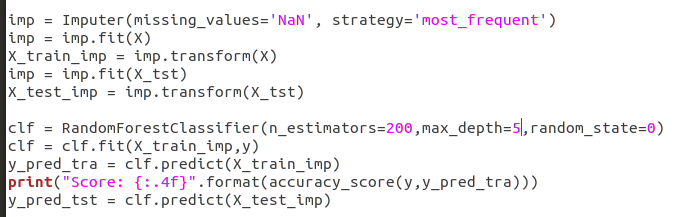
\includegraphics[scale=0.5]{rfimp.png}  %el parámetro scale permite agrandar o achicar la imagen. En el nombre de archivo puede especificar directorios
	\caption{Prueba con RF imputando MV} 
	\label{fig:RF1}
\end{figure}

\begin{figure}[H] %con el [H] le obligamos a situar aquí la figura
	\centering
	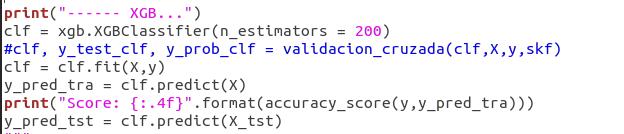
\includegraphics[scale=0.6]{xgb1.png}  %el parámetro scale permite agrandar o achicar la imagen. En el nombre de archivo puede especificar directorios
	\caption{Prueba con XGB} 
	\label{fig:xgb1}
\end{figure}

Los algoritmos generaban resultados pobres fruto del nulo preprocesamiento de datos. 

\section{Solución 1}

Lo primero que hice, ya de forma más seria, fue un análisis exploratorio de los datos. También dibujé la distribución de las tres clases:

\begin{figure}[H] %con el [H] le obligamos a situar aquí la figura
	\centering
	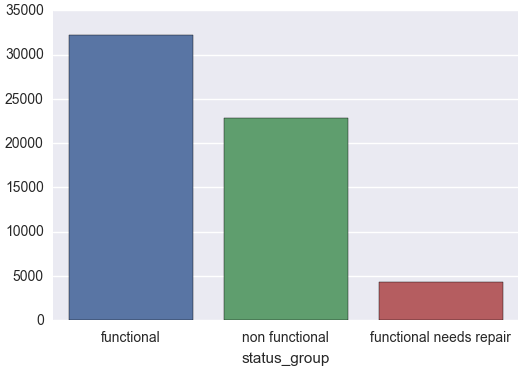
\includegraphics[scale=0.5]{clases.png}  %el parámetro scale permite agrandar o achicar la imagen. En el nombre de archivo puede especificar directorios
	\caption{Distribución de las clases} 
	\label{fig:CLASES}
\end{figure}

Tras el análisis exploratorio, extraje las siguientes conclusiones:

\begin{enumerate}
	\item La mayoría de las variables son categóricas
	\item Ciertas variables poseen un porcentaje elevado de 'null', lo que va a requerir de una imputación.
	\item La mayoría de las variables categóricas tienen grandes cantidades de valores únicos.
	\item Existe redundancia entre las variables
\end{enumerate}

\begin{figure}[H] %con el [H] le obligamos a situar aquí la figura
	\centering
	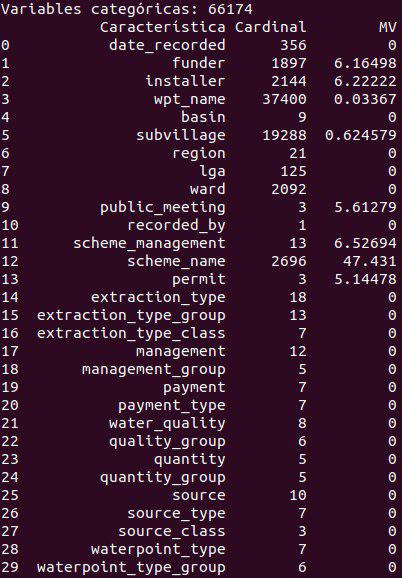
\includegraphics[scale=0.5]{categoricas.jpg}  %el parámetro scale permite agrandar o achicar la imagen. En el nombre de archivo puede especificar directorios
	\caption{Categóricas y porcentaje de MV} 
	\label{fig:cat}
\end{figure}

Por tanto, a pesar de que las clases están desbalanceadas, la mayoría de mi preprocesamiento se basará en seleccionar y modificar características.

\subsection{Tratamiento de características}

De entre las pocas variables numéricas que tenemos, se observa que muchas de ellas presentan valores perdidos. En concreto, para \textit{longitude}, \textit{latitude}, \textit{gps\_height} y \textit{population}, los valores nulos y ceros son estimados a través de la media para \textit{district\_code}, \textit{basin} y \textit{subvillage}:

 \begin{figure}[H] %con el [H] le obligamos a situar aquí la figura
 	\centering
 	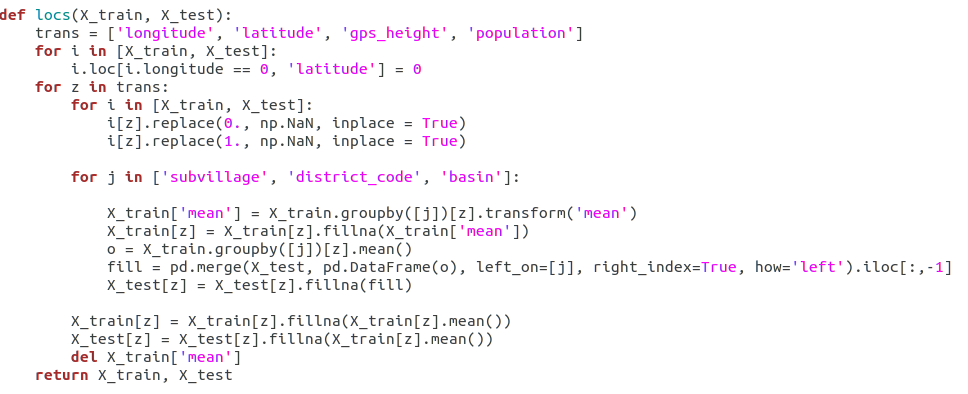
\includegraphics[scale=0.42]{locs1.png}  %el parámetro scale permite agrandar o achicar la imagen. En el nombre de archivo puede especificar directorios
 	\caption{Tratamiento de null y 0} 
 	\label{fig:locs1}
 \end{figure}

Por otra parte, reduzco la dimensionalidad utilizando PCA sobre las variables continuas \textit{longitude}, \textit{latitude} y \textit{gps\_height}

 \begin{figure}[H] %con el [H] le obligamos a situar aquí la figura
	\centering
	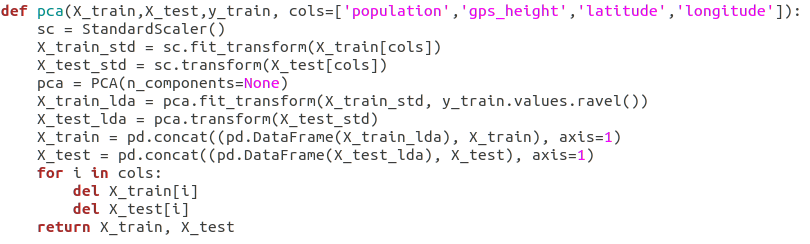
\includegraphics[scale=0.45]{pca1.png}  %el parámetro scale permite agrandar o achicar la imagen. En el nombre de archivo puede especificar directorios
	\caption{PCA sobre variables continuas} 
	\label{fig:pca1}
\end{figure}

Por otra parte, elimino un gran número de columnas por la redundacia encontrada:

 \begin{figure}[H] %con el [H] le obligamos a situar aquí la figura
	\centering
	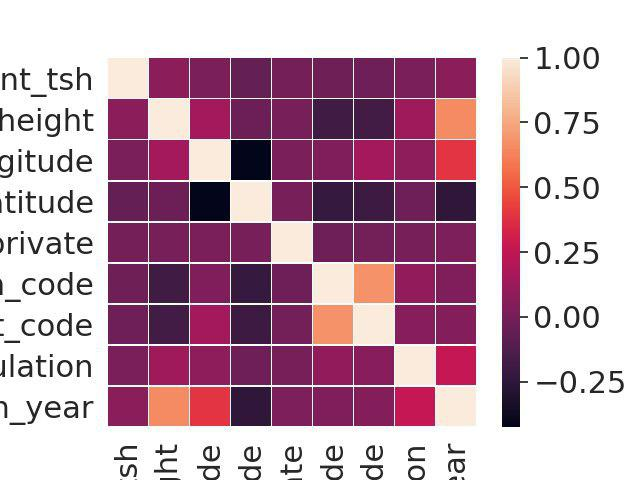
\includegraphics[scale=0.4]{correlaciones.png}  %el parámetro scale permite agrandar o achicar la imagen. En el nombre de archivo puede especificar directorios
	\caption{Correlación entre variables numéricas} 
	\label{fig:correlaciones}
\end{figure}

Por tanto, elimino las variables \textit{id}, \textit{amount-sh}, \textit{num-private}, \textit{region}, \textit{quantity}, \textit{quality-group}, \textit{source-type}, \textit{payment}, \textit{waterpoint-type-group}, \textit{extraction-type-group} y \textit{scheme-name}.

Por último, convierto el resto de variables categóricas en dummies para poder operar con ellas.

\subsection{Ajuste de hiperparámetros}

Ajusto el número de estimadores (500,750 o 1000) para mi modelo. He probado distintas configuraciones (explícitas en la tabla superior) en función de también ligeras modificaciones en el preprocesamiento. De las 25 entregas, muchas de ellas han sido cambiando parámetros, por lo que no subo una copia del código por cada modificación.

 \begin{figure}[H] %con el [H] le obligamos a situar aquí la figura
	\centering
	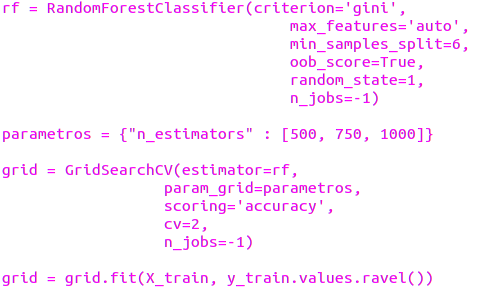
\includegraphics[scale=0.4]{grid.png}  %el parámetro scale permite agrandar o achicar la imagen. En el nombre de archivo puede especificar directorios
	\caption{Ajuste de hiperparámetros con GridSearch} 
	\label{fig:grid}
\end{figure}

\newpage

\subsection{Modelo}

Tras el ajuste, tenemos el siguiente modelo:

 \begin{figure}[H] %con el [H] le obligamos a situar aquí la figura
	\centering
	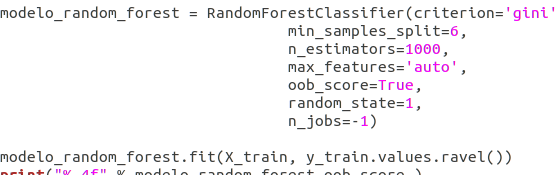
\includegraphics[scale=0.4]{rf.png}  %el parámetro scale permite agrandar o achicar la imagen. En el nombre de archivo puede especificar directorios
	\caption{Random Forest} 
	\label{fig:RF}
\end{figure}

 
\section{Solución 2}

Buscando un ensemble learner en la documentación, encontré CatBoost (\cite{catboost1}). A pesar de que los resultados no fueron buenos (y menos aún al aplicar el mismo preprocesamiento para XGB), parece enriquecedor aquí señalarlo puesto que para mí fue un aprendizaje.  

Tras limpiar los datos eliminando variables por irrelevantes o por tener demasiados niveles, cambiando los NAN para poder computar, cambiar tipos y escalando características numéricas,

\begin{figure}[H] %con el [H] le obligamos a situar aquí la figura
	\centering
	\includegraphics[scale=0.4]{prep2.png}  %el parámetro scale permite agrandar o achicar la imagen. En el nombre de archivo puede especificar directorios
	\caption{Seleccionando características e impuntando valores perdidos} 
	\label{fig:prep-cat1}
\end{figure}

\begin{figure}
	\centering
	\includegraphics[scale=0.4]{prep21.png}  %el parámetro scale permite agrandar o achicar la imagen. En el nombre de archivo puede especificar directorios
	\caption{Conversión de tipos} 
	\label{fig:prep-cat2}
\end{figure}



 utilizo CatBoostClassifier con los siguientes parámetros: 

\begin{figure}[H] %con el [H] le obligamos a situar aquí la figura
	\centering
	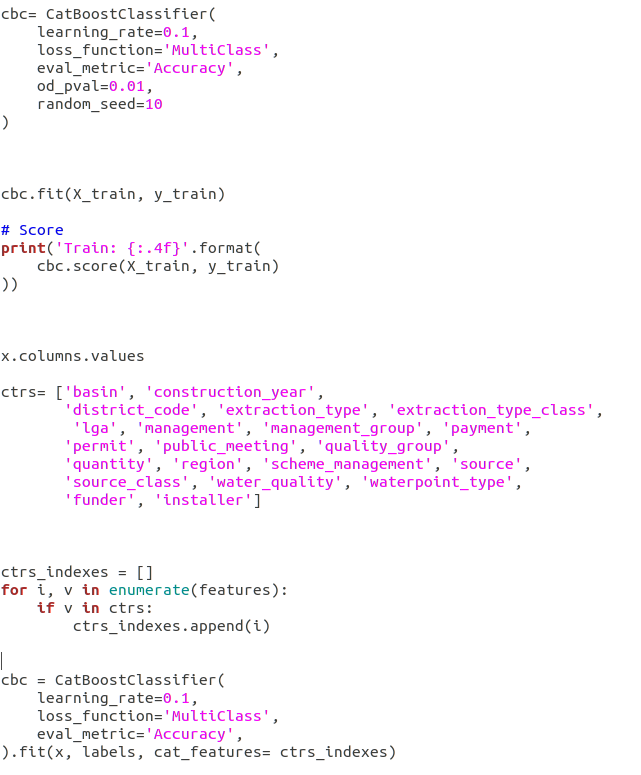
\includegraphics[scale=0.32]{catboost1.png}  %el parámetro scale permite agrandar o achicar la imagen. En el nombre de archivo puede especificar directorios
	\caption{CatBoost} 
	\label{fig:CB1}
\end{figure}


Con los mismos datos pruebo dos configuraciones de parámetros distintas de XGB con resultados muy pobres.

\begin{figure}[H] %con el [H] le obligamos a situar aquí la figura
	\centering
	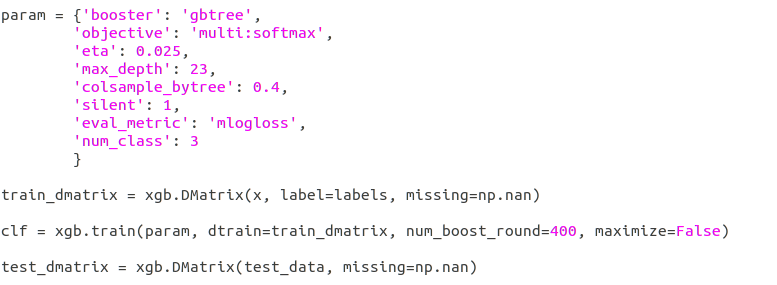
\includegraphics[scale=0.5]{xgb2.png}  %el parámetro scale permite agrandar o achicar la imagen. En el nombre de archivo puede especificar directorios
	\caption{XGB (1)} 
	\label{fig:xgb2}
\end{figure}

\begin{figure}[H] %con el [H] le obligamos a situar aquí la figura
	\centering
	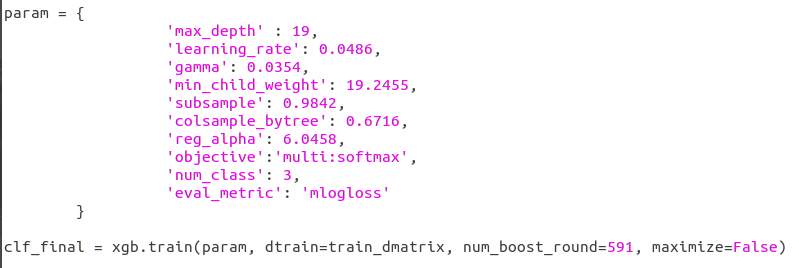
\includegraphics[scale=0.5]{xgb3.png}  %el parámetro scale permite agrandar o achicar la imagen. En el nombre de archivo puede especificar directorios
	\caption{XGB (2)} 
	\label{fig:xgb3}
\end{figure}

\newpage

\section{Solución 3}

Es la solución 3 la que me da el mejor resultado. Presentía que el problema, como casi siempre, es el preprocesamiento y con Python no acababa de ver con facilidad el conjunto de datos. En un intento de mejorar, cambio a R (consultando \cite{r2}, \cite{r1}) y comienzo de (casi) cero el problema. Con las ideas que me han ido dando las demás visualizaciones y, francamente, tirando de sentido común más que de conocimiento real, elimino 24 de las 40 variables disponibles porque considero (también lo vi antes con el gráfico de correlaciones) con muchas de ellas son redundantes. 

\begin{figure}[H] %con el [H] le obligamos a situar aquí la figura
	\centering
	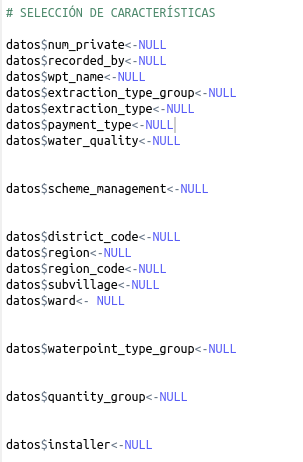
\includegraphics[scale=0.6]{selec-carac.png}  %el parámetro scale permite agrandar o achicar la imagen. En el nombre de archivo puede especificar directorios
	\caption{Selección de características} 
	\label{fig:selec-carac}
\end{figure}



Además, como se ve en la imagen anterior, elimino más variables dado que, tras ejecutar el modelo, estudio la importancia de las mismas:


\begin{figure}[H] %con el [H] le obligamos a situar aquí la figura
	\centering
	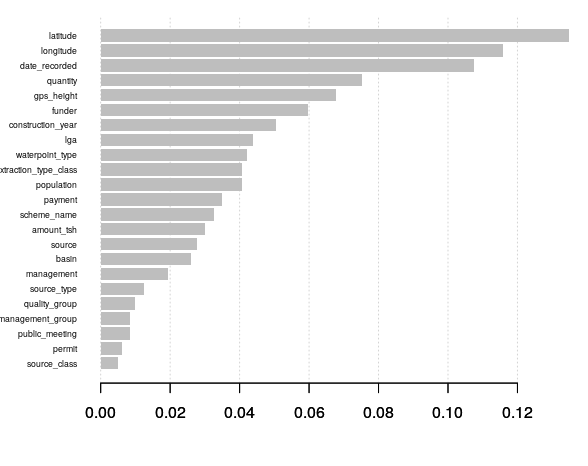
\includegraphics[scale=0.7]{importancia-variables.png}  %el parámetro scale permite agrandar o achicar la imagen. En el nombre de archivo puede especificar directorios
	\caption{Importancia de las variables en el modelo} 
	\label{fig:importancia}
\end{figure}

Por otra parte, imputo valores para las variables construction-year y gps-height utilizando la mediana de los datos que sí son validos en sendas columnas. 

\begin{figure}[H] %con el [H] le obligamos a situar aquí la figura
	\centering
	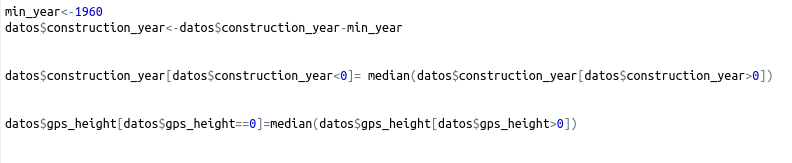
\includegraphics[scale=0.5]{mv.png}  %el parámetro scale permite agrandar o achicar la imagen. En el nombre de archivo puede especificar directorios
	\caption{Imputación en las variables construction-year y gps-height} 
	\label{fig:mv}
\end{figure}




Una vez que están preparados los datos, construyo un ensemble con entre 11 y 25 modelos XGBoost de igual peso en la solución. Digo 25 porque entre las distintas entregas he ido cambiando parámetros y 25 me propinó los mejores resultados. Además, utilizó validación cruzada para delimitar el número de iteraciones realmente útiles (una vez que se deja de obtenerse ganancia, no sigo iterando) y genero el modelo con los mismos parámetros (también los he cambiado, como expreso en la tabla superior) y lo predigo con ese modelo los distintos valores de test. Esas predicciones las voy acumulando en columnas de la tabla \textit{solucion}.

\begin{figure}[H] %con el [H] le obligamos a situar aquí la figura
	\centering
	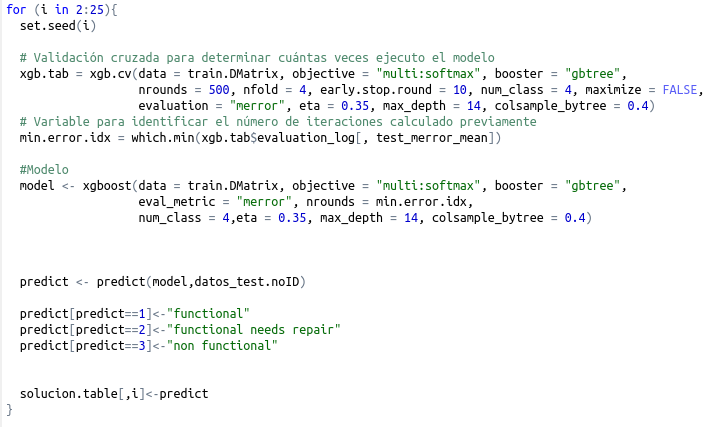
\includegraphics[scale=0.5]{modelo-ensemble.png}  %el parámetro scale permite agrandar o achicar la imagen. En el nombre de archivo puede especificar directorios
	\caption{Bucle con CV y la creación del modelo con los mismos parámetros} 
	\label{fig:modelo}
\end{figure}

Por último, agrupo la tabla solución en un vector contabilizando los resultados más repetidos para cada fila. Tras ello, genero la predicción en el formato correspondiente para la entrega y la envío. 

\newpage
 
\section{Bibliografía}

%------------------------------------------------

\bibliography{citas} %archivo citas.bib que contiene las entradas 
\bibliographystyle{plain} % hay varias formas de citar

\end{document}
